\section{The Approach}
\label{sec:approach}


Causal relation exists between an event and another event or factor and phenomenon.
Generally, cause and effect can be changes, events, processes, properties, processes, facts, states and so on.
Therefore the parts of speech(POS) may be verb, noun, adjective or adverb.
We focus on finding the causality among all types of words mentioned before.
Our approach simply follows three steps.
First, we extract candidate pairs which include the cause and effect word as well as the times the pair has ever appeared in corpus.
Second, we extract some features including sementic, graphic and statistic features from the pairs and the statical data.
And finally, we employ a learning algorithm to classify each of the pair to either a true causal relation or not.

%Causal relation exists between two events, one being the cause, and the
%other being effect. We focus on noun phrase causality which
%both the cause and the effect are noun phrases. Our approach generally
%follows three steps. First, we extract candidate triples which include the
%cause, the effect, and a text span that contains the causal cue patterns
%between the two events. The {\em text span} is defined as the string between
%the two noun phrases. Second, we extract some crucial features from
%the triples as alternate representations. And finally,
%we employ a learning algorithm to classify
%each of the triples to either a true causal relation or not.

\subsection{Causal Candidates Extraction}
\label{sec:extract}

\begin{table*}[t]
\small
\begin{center}
\begin{tabular}{|c|c|}
\hline
\multicolumn{2}{|c|}{Cue Patterns}\\
\hline
A lead to B & A leads to B\\
A led to B & A leading to B\\
A give rise to B & A gave rise to B\\
A given rise to B & A giving rise to B\\
A induce B & A inducing B\\
A induces B & A induced B\\
A bring on B & A bringing on B\\
A brings on B & A brought on B\\
B result from A & B resulting from A\\
B results from A & B resulted from A\\
If A , then B & If A , B\\
B , because A & B because A\\
B because of A & Because A , B\\
A , thus B & A , therefore B\\
B as a result of A &Inasmuch as A , B\\
B , inasmuch as A & Due to A , B \\
B due to A & In consequence of A , B \\
B in consequence of A & B as a consequence of A\\
B , A as a consequence & As a consequence of A , B\\
B owing to A & Owing to A , B\\
A , hence B & A and hence B \\
A , consequently B & A and consequently B \\
A , for this reason alone , B & B caused by A\\
A caused B & A causes B \\
A causing B & A cause B \\
a/the/one effect of A is/are/was/were B & the reason(s) for/of B is/are/were/was A\\
A is/was/are/were a/the/one reason(s) of/for B & \\
\hline
\end{tabular}
\end{center}
\caption{\label{table:patterns} Patterns used to extract candidate pairs. }
\end{table*}

In order to extract causal candidates from open domain text, several cue patterns are used here.
{\em Cue patterns} which is composed of discourse marker and predicate pattern are the words that imply the probability of existence of causal relation.
{\em Discourse marker} is always the connectives. It splits a sentence into two complete sub sentences such as \textquotedblleft because\textquotedblright \, and \textquotedblleft if \ldots then \ldots \textquotedblright.
{\em Predicate word} is always a verb or verb phrase, such as \textquotedblleft lead to\textquotedblright \ and \textquotedblleft give rise to\textquotedblright \ .
Sentences contain predicate words are usually separated into two incomplete parts.
Patterns we used are shown in Table \ref{table:patterns} and are considered to be strong and comprehensive enough to indicate the existence of causal relation.

Sentences containing those patterns are extracted first.
Each sentence is then divided into two parts by the pattern. Actually, we just remain 10 words in each part because we argue that words far away from the cue pattern carry little information about causal relation.
We assume that the former part contains the cause word and the latter one has the effect word.
Words are splitted and filtered because some words are useless and may even bring noises such as \textquotedblleft about\textquotedblright, \textquotedblleft after\textquotedblright, \textquotedblleft the\textquotedblright, which we call {\em stop words}.
Always, we check whether the word is in WordNet. If not, we drop it.
Finally, every word before the cue pattern is roughly connected to every word after it to form the candidate pairs.
The corresponding cue pattern and the count of the pair is also
recorded and accumulated.  So, what we get at last is like
Table \ref{table:candidate}.
\begin{table}
\small
\begin{center}
\begin{tabular}{|c|c|c|c|}
\hline
cause & effect & ... pattern frequency ... & total frequency \\
\hline
\end{tabular}
\end{center}
\caption{\label{table:candidate}Candidate Pair's Form }
\end{table}
Cause and effect correspond to the candidate cause and effect words respectively. Pattern frequency related to different cue patterns. It records the frequency the pair shows up together with one certain pattern. Since we use 53 patterns, 53 number is recorded for each pair. Total frequency is the sum of the former pattern frequency.


%we first employ the open information extraction system Reverb
%\cite{BankoCSBE07} to extract all relation triples that satisfy one of
%the 71 causal cue patterns which were previously reported by
%Girju et al.\cite{girju2003automatic}. We extract causal text span
%and noun-phrase chunkers together. Then we filter out those chunkers whose
%head word are not included in WordNet\cite{wordnet}.
%At this point, we obtain the causal candidates from text.
%The candidates are the triples in the following form:
%\triple{$NP1$}{$cue$}{$NP2$}, where {\em cue} stands for the
%causal cue pattern such as ``cause'', ``lead to'', etc. For example,
%from sentence A-2 in Section
%\ref{sec:intro}, we can get the causal candidate triple as follows:
%\triple{acid\_rain}{contribute\_to}{corrosion\_of\_metals}.
%We may get more than one triple from each sentence.


\subsection{Feature Extraction}
\label{sec:features}

In Section \ref{sec:extract}, we obtained the causal candidates by causal cue patterns in which case we take both the correlation and causality into consideration.
Based on that, we then extract features from three angles: statistic, graphic and semantic.
Semantic features pay more attention to words' meanings since the causal relationship exists in the semanteme itself.
Graphic features concentrate on the relations among pairs. Some common structures are used as feature here.
Statistic features focus on the mathematical process such as frequency, standard deviation and so on.



\subsubsection{Semantic Features}
\begin{table*}[t]
\small
\begin{center}
\begin{tabular}{|c|c|c|}
\hline
\multicolumn{3}{|c|}{Categories}\\
\hline
thing.n.08 & matter.n.03 & process.n.06\\
motivation.n.01 & causal\_agent.n.01 & keepsake.n.01\\
whole.n.02 & web.n.01 & ribbon.n.01\\
geological\_formation.n.01 & land.n.04 & thing.n.12\\
land.n.04 & film.n.04 & curio.n.01\\
charm.n.03 & part.n.02 & location.n.01\\
remains.n.01 & riviality.n.03 & stuff.n.02\\
communication.n.02 & group.n.01 & attribute.n.02\\
set.n.02 & measure.n.02 & relation.n.01\\
quality.n.03 & cognition.n.01 & event.n.01\\
feature.n.01 & & \\
\hline
\end{tabular}
\end{center}
\caption{\label{table:category} 31 Categories from WordNet }
\end{table*}

It is natural to think that causality is more concerned with semantic meaning rather than grammatical rules.
Three reasons are shown here that why we extract semantic features:
\begin{itemize}
\item A word can have a lot of different meanings. In many cases, whether a pair of word has causality relationship depends on the context to a great extent. When judging a causality relationship, we need to combine the word with the specific environment to determine which meaning the word is. There is no doubt that the word's meaning will make a big difference in deciding the relationship.
\item The POS of words may also influence the judgment. Our goal is to find causality relationship in whole text. Not only the causality between nouns but also the causality between verbs, adjectives, adverbs and between each other. Therefore, it is rather important to fetch the POS information of words, which can also be classified into semantic feature.
\item Different categories of words have differences in causing different thing. From this point of view, we need to classify all nouns into several categories and the certain category for a certain word can be a simple and crude symbol which can be used to represent the feature of meaning. Besides the categories also provide us with another point of view to evaluate the confidence of the causality between a pair of words.  For example, \textquotedblleft motivation\textquotedblright \ and \textquotedblleft film\textquotedblright \ are two categories in our final set of category. Compared with \textquotedblleft motivation\textquotedblright \ , \textquotedblleft film\textquotedblright \ is much more likely to cause changes in \textquotedblleft emotion\textquotedblright \ . On the contrary, \textquotedblleft motivation\textquotedblright \ will contribute more to a result of \textquotedblleft action\textquotedblright \ than \textquotedblleft film\textquotedblright \ . In a word, probability for causality is associated with the category that cause and effect words belong to.
\end{itemize}

Senmantic information is an important feature but hard to extract. In our experiment, WordNet and Google N-gram are two main corpuses used here.
WordNet has a tree structure and there is always a shared hypernyms for any two words.
The higher level the word is, the more words will converge on it.
Therefore, we investigate the structure of the tree and find out 31 top-level words to represent all categories which are showed in Table \ref{table:category}.
The 31 categories can cover most of the words in WordNet which in turn means most of the words can be classified into these 31 categories.
Most semantic information for noun can be extracted from hypernyms directly while the semantic feature for verbs, adjectives, and adverbs needs to be found in context. We believe that the object and subject for a verb or the word modified by an adjective or an adverb contains more useful and significant information. Google N-gram is a contiguous sequence of n items from a given sequence of text or speech from natural language. To be specific, we use the Google 2-gram corpus in our experiment to find those significant words by the following steps:
\begin{itemize}
\item For verbs: We extract all the objects and subjects of a certain verb. To extract objects, two situations must be included. The first is direct object, the noun phrase which is the accusative object of the verb. For example, from the sentence \textquotedblleft Smoking causes cancer.\textquotedblright \ we can know the  \textquotedblleft cancer \textquotedblright \ is a direct object of cause.  The second situation needs to be taken into consideration is the passive nominal subject. Once again, let��s take \textquotedblleft smoke\textquotedblright \ and \textquotedblleft cance\textquotedblright \ as example. At this time the sentence is changed to \textquotedblleft Cancer can be caused by smoke\textquotedblright \, the cancer is the passive nominal subject and it's actually the object of cause. For subject, the main situation needs to be considered is just the same as object.
\item For adjectives: We extract the modified nouns of the adjective to have a better understanding about where the adjective is mostly used. For example, we will get the word \textquotedblleft algorithm\textquotedblright \ for adjective \textquotedblleft powerful \textquotedblright \ in the 2-gram \textquotedblleft powerful algorithm\textquotedblright \ .
\item For adverbs: We extract the modified words for adverb just like adjective. For example, we will get the core modified word \textquotedblleft speaking\textquotedblright \ for adverb \textquotedblleft generally \textquotedblright \ from the 2-gram \textquotedblleft generally speaking\textquotedblright \ .
\end{itemize}


Those significant words share some similarities. First, there is a dependency between the significant words and the original one. Second, those words are all nouns and can be classified into 31 categories.
The categories of the significant words represent the categories of the original word. Frequency is also recorded because one word can have many significant words so it can be classified into several categories.

When a new word comes from original corpus, our processing procedure is showed in Figure \ref{fig:flow}.

\begin{figure}[th]
\centering
\epsfig{file=flowchart.eps, width=\columnwidth}
\caption{Flowchart for semantic feature}
\label{fig:flow}
\end{figure}

 In general, WordNet is mainly used to classify words into different categories and extract the information concerning the meaning of the word while Google N-gram, on the other hand, is mainly used to get the information of the position and possible position for a word in the context, which can be used to analyze different combination and collocation for each certain word.
We can say that Wordnet is used to extract features for nouns while Google N-gram is used for verbs, adjectives and adverbs.

\subsubsection{Graphic Features}
\begin{figure*}[th]
\centering
\begin{subfigure}[h]{0.7\columnwidth}
\centering
\epsfig{file=sibling1.eps,width=\columnwidth}
\caption{Sibling Structure}
\label{fig:sibling}
\end{subfigure}
\hfill
\begin{subfigure}[h]{0.8\columnwidth}
\centering
\epsfig{file=loop.eps,width=\columnwidth}
\caption{Loop Structure}
\label{fig:loop}
\end{subfigure}
\hfill
\begin{subfigure}[h]{0.3\columnwidth}
\centering
\epsfig{file=closure.eps,width=\columnwidth}
\caption{Closure Structure}
\label{fig:closure}
\end{subfigure}
\caption{Graphical Features}
\label{fig:graph}
\end{figure*}

Though the most intuitive impression of causality relation comes from the context, the statistic data and the graphic features are of great importance in preventing the result from being affected by the subjective impression and make the most use of original corpus.

Imagine the words as nodes and the causal relations between two words as lines, all those above form a huge causal net.
It is natural to believe that some structures do have meanings to the causal relation.
We combine the simple \{0, 1\} label together with the frequency label to describe the feature.

\begin{enumerate}[1)]
\item {\em Sibling Structure}\\
Sibling structure considers the situation where pairs share the same cause or effect.
There are actually two types of sibling structure as is shown
Figure \ref{fig:sibling}.
For example, pairs $<$lack, reduce$>$.
There are many pairs with candidate cause word being \textquotedblleft lack\textquotedblright \, so
one feature here is used to indicate this pair does exist in such structure and another feature records the total number of effects when the \textquotedblleft lack\textquotedblright \ is used as cause. It is reasonable to believe that some words have high possibility to be a cause word or effect word. And, the neighbour amount of the other word will relatively be larger. In another word, the second feature of this pair here evaluates the cause word's weight.
\item {\em Loop Structure}\\
Loop structure also consists of two types. It exists between 2 words or among 3 words. Figure \ref{fig:loop} shows the two types of loop structure:
The line with arrow starts from the word that we think is cause word and ends to the word which we believe to be an effect word.
Obviously, Type I describes the loop relationship between two words.
It is acceptable that few causal pairs may exist in such structure where A causes B and B causes A. Some examples that show no causal relation is as follows: $<$lack, controversy$>$, $<$lack, projection$>$, $<$lack, music$>$ and so on.
As the same, Type II depicts the relation among three words. A few more pairs may exist in such structure but we still prefer to believe pairs in such structures are less reliable.
\item {\em  Closure Structure}\\
Closure structure exists among three words. Any two words of the three are
supposed to have causal relation. Its structure is shown in
Figure \ref{fig:closure}.
There are three pairs here: $<$Word1, Word2$>$, $<$Word2, Word3$>$, $<$Word1, Word3$>$. It is an ideal structure because if there exists causal relation in the former two pairs, we may strongly believe that the third pair also has the same relation. The causal relationship is enhanced here. It is worth mentioning that different positions of the pairs in the triangle may have different meanings so we use three-bit feature to describe it.
\end{enumerate}

\subsubsection{Statistic Features}
We extract the statistic features on the basis of the following three hypothesis:
\begin{description}
\item[H1] The frequency positively affect the possibility of causal relation.
\end{description}
Since we filter the stop words, it is for sure that remaining words are meaningful. Pairs with low frequency means either the causality doesn't exist or the causality is rare and weak. On the other hand, pairs with high frequency implies the correlation or causality is widely recognized and the probability of the causality is higher.
\begin{description}
\item[H2] The smaller standard deviation of pattern distribute, the more possibility of causality.
\end{description}
It is apparently that one pair is strongly causal if most patterns contribute to \textquotedblleft prove\textquotedblright \, the causality. All the patterns we use are at least has the function of implying the existence of causality. If one pair is found together with most patterns, we have the reason to believe that the two words have high probability to be causal relation. Under this condition, deviation will be a good feature to evaluate the distribution of the pattern frequency.
%For example, the distribution of different pattern of pair $<$disease, death$>$ is 1100 : 410 : 270 : 548 : 9 : 2 : 0 : 0 : 12 : 29 : 55 : 23 : 1 : 0 : 2 : 6 : 159 : 404 : 48 : 220 : 16 : 86 : 135 : 301 : 334 : 58 : 35 : 23 : 413 : 0 : 0 : 12 : 8896 : 0 : 5 : 20 : 3 : 0 : 45 : 0 : 12 : 5 : 8 : 5 : 0 : 2638 : 1532 : 7969 : 948 : 23358 : 17 : 15 : 11. Almost all patterns are found to be in sentences together with the word \textquotedblleft disease\textquotedblright \, and \textquotedblleft death\textquotedblright. So the pair is more likely to have causal relation.

\begin{description}
\item[H3] Different cue patterns makes different contribution to \textquotedblleft prove\textquotedblright \ the causality of the pair.
\end{description}
 Even if we believe our pattern is strong and efficient, there is still some differences between those patterns. Some patterns may have two meanings like \textquotedblleft contribute to \textquotedblright \ . It not only has the causal meaning but also has the meaning of \textquotedblleft devotion \textquotedblright \ . Some patterns predict the causality in a implicit way, such as\textquotedblleft if A, B\textquotedblright \ . In this case, some patterns may predict strong causality while others predict weaker one. We use the pattern frequency here to describe the feature which evaluate the pattern of the pairs.
%\begin{equation}
%pair\_weight = existence\_count * pattern\_weight
%\end{equation}
%Clearly, each pair has 53 pair\_weight features.

Above all, we extract frequency, standard deviation as feature and pattern score features,
which can be used to represent the candidate pairs.



\subsection{Learning Algorithm}
\label{sec:learning}
In this part, we build a classifier to identify true causal relations in the candidate pairs.
The Restricted Boltzmann Machin(RBM) which is now often used to build deep belief networks(DBNs) provides a good initialization for feed-forward neural networks. It has been used in a variety of application domains successfully.
However, it is always used in feature reduction for other learning algorithm or used as an unsupervised learning method.
In the last layer of a DBM, RBM can model the joint distribution of the inputs and associated target classes rather than only model the inputs(e.g. in the last layer of a Deep Belief Network in Hinton et al. (2006))
As a matter of fact, RBM can also be used to do the classification itself and may perform better than SVM or neural network.
The Model is shown in Figure \ref{fig:RBM}:

\begin{figure}[th]
\centering
\epsfig{file=RBM.eps, width=\columnwidth}
\caption{RBM model}
\label{fig:RBM}
\end{figure}

In this model, h is the hidden layer, x is  the visible layer that we can observe and y relates to the target class.
Suppose we have m hidden units, n visible units and he number of classes is C, then $h = \{h_1, h_2, ..., h_m\}$ and $x = \{x_1, x_2, ..., x_n\}$
Denote the training set is $\mathscr{D}$ = {(x$_i$,y$_i$)}, where x$_i$ is the feature of the \textit{i}-th example and y$_i$ $\in $
$\mathscr{R}$ $^C$.
So the energy function is:
\begin{equation}\nonumber
\begin{aligned}
E(y,x,h) &= -h^TWx-b^Tx-c^Th-d^Ty-h^TUy
\end{aligned}
\end{equation}
With the parameters $\theta = (W,\, b,\, c,\, d,\, U)$.
And the probability distribution function is:
\begin{equation}\nonumber
\begin{aligned}
p(y,x,h) &= \frac{1}{Z}e^{E(y,x,h)}
\end{aligned}
\end{equation}
where Z is the normalization coefficient.
Our goal is to minimization of the negative log-likelihood:
\begin{equation}\nonumber
\begin{aligned}
L(D) &= -\sum\nolimits_{i=1}^{|D|} \log{p(y^{(i)}, x_i)}
\end{aligned}
\end{equation}
$y^{(i)}$ is the \textit{i}-th class of the C classes and $|D|$ is the number of examples.


%\subsubsection{Data Set}
%
%We use the Wikipedia articles as our corpus. After the preprocessing and
%filtering step in Section \ref{sec:extract}, we obtained 5754 candidate triples.
%We select 200 instances and manually classified them as ``causal'' or
%``non-causal''. We take 150 out of 200 instances as the training set,
%and take the other 50 instances as the test set.

%\subsubsection{Supervised Learning Method}
%
%Our first attempt of a supervised learning method uses a linear model
%to combine
%the numeric features. The linear classifier is defined as follows:
%\[s(t) = \sum\limits_{i = 1}^4 {w_i*f_i} \]
%where $s$ is the metric value of the triple $t$, $f_i$ is the feature
%of the triple $t$, and $w_i$ is the weights of $f_i$.
%To solve the model, we only need to get the weights $w_i$ and the
%threshold $m$. We use the threshold to classify triples. For triple
%$t=$\triple{$np_i$}{$cue$}{$np_j$}, if $s(t) \ge m$, we take
%\pair{$np_i$}{$np_j$} as causal pair, otherwise we reject this pair
%as non-causal. To this end, we use the simulated annealing algorithm
%\cite{KirkpatrickGV83}
%to search for a reasonable solution ($w_1$, $w_2$, $w_3$, $w_4, m$).
%%We train the parameters with the training set built in Section 3.3.1, and evaluate the model on the test set.
%
%Since the features we extract are all numeric, we further adopt
%an implementation of Logistic Regression model\cite{witten2005data} to build the classifier.
%%We compare our proposed models to previous work
%%(Girju et al., 2003; Chang and Choi, 2006) on the same dataset.
%%The results are showed in table1.
%
%\subsubsection{Unsupervised Learning Method}
%
%The annotated work for supervised models is time consuming and cannot scale up.
%We next propose an unsupervised method to solve this problem.
%Our inspiration comes from Chang and Choi\cite{chang2006incremental}.
%Generally speaking, we embed our causal association metrics model
%into an EM algorithm. During each iteration, we update the model parameters
%in E-step, and classify the candidates in M-step until the parameters converge.
% We built the initial classifier with $pmi$ feature only.
%The top 45\% of triples are classified into ``causal'', and the rest are
%classified into ``non-causal''. Then, for the following classification of
%each iteration, we reconstruct a Naive Bayesian Classifier
%with new parameters. The class $c$ of triple $t$ is computed as follows:
%
%\[c = \mathop {\arg \max }\limits_{c_k} P(c_k|t_i) = \mathop {\arg \max }\limits_{c_k} \frac{{P(c_k)P(t_i|c_k)}}{{P(t_i)}}\]
%
%We assume that all the causal features are independent.
%In our model, $P(t_i|c_k)$ can be rewritten as:
%\[P(t_i|c_k) = p(ccpt_i|c_k)\prod\limits_{j = 1}^4 {P(t_i(f_j)|c_k)} \]
%where $t_i(f_j)$ gives the $j$th numeric feature value of triple $t_i$,
%and $cppt_i$ is the causal cue phrase of triple $t_i$.
%We define the $P(t_i(f_j)|c_k)$ as follows:
%
%\[P(t_i(f_j)|c_k) = \frac{{freq(\forall t_x(f_j) \in \theta (t_i(f_i)))}}{{freq(\forall t_x \in c_k)}}\]
%where $t_x$ presents the arbitrary triple, \(\theta (t_i(f_i))\) gives an interval which $t_i(f_i)$
%belongs to. The range of each feature is pre-divided into 10 intervals,
%so that they would not change in each iteration.

